\chapter{Residual risks}
In this last chapter are presented some important best practices along with a deep analysis of the common attacks on \textit{OAuth2}. All the risks linked to the protocol are described in the Section 10 of the RFC-6749 \cite{RFC6749}.

\minitoc

\section{Introduction}
Just as with any application, security should be a top priority. This is especially true for applications that utilize this protocol. In order to understand why it is true, could be helpful to summarize what OAuth2 does. Recalling that, it has been discussed how OAuth2 provides federated identity as well as delegated authority. If there is no diligence with security practices during the implementation, some very dangerous holes can be exposed for attackers to exploit.
Indeed, when dealing with federated identity and delegated authority (since these are very powerful practices that can provide attackers with a lot of power) the developers must be extra vigilant.

If an attacker were somehow able to exploit an application to game either of these concepts, they may be able to do the following:

\begin{itemize}
    \item Impersonate users
    \item Impersonate client applications
    \item Grant themselves otherwise unauthorized permissions
    \item Gain access to protected data and resources
\end{itemize}

In order to fight this, there must be extra carefulness with the implementation with regard to the client integration with the service provider via OAuth2. 

\section{Best practices}
There are surely countless ways that a given application can be exploited. The objective is to minimize the attack vectors available to attackers, but it is not possible to cover all the possibilities. What follows is a non-exhaustive list of security best practices that will help to keep an application as secure as possible. 

\subsubsection{Use the authorization code grant flow}
The authorization code grant flow is by far the most secure flow available. It utilizes a back-end server to securely store and transmit sensitive properties, such as client credentials and tokens, to and from the service provider.
Proper use of a server to facilitate these communications will completely abstract, and hide, the flows from the end-user, as well as any attackers.

\subsubsection{Use TLS}
It might seem like an obvious tip, but it is important enough to note. The use of secure communication channels applies for when the client application talks to service providers, as well as when the service providers talk to the client application. When a client application talks to the service provider, it does so by interacting with their authorization and token endpoints. It must be ensured that they utilize TLS so that the communication with them is secure and encrypted.

Additionally, when the service provider talks back to the client application, it does so via the redirect URI that has been previously passed to it. Even this endpoint, owned by the developer, must utilizes TLS as well.

\subsubsection{Use the refresh token}
For clients using the authorization code grant flow, depending on the service provider, a refresh token may be returned to the client. When an access token expires for a user, rather than requiring them to authenticate again, the refresh token can be used to request a new, valid access token. This is desirable from both a security standpoint as well as a usability standpoint.

In terms of security, the fewer times a user has to authenticate means the fewer times a user has to send their username and password across the Internet. This also means fewer opportunities for an attacker to steal them.

From a usability standpoint, this means that the application can function for longer periods of time without having to ask the users to re-log in.

\subsubsection{Use native browsers}
\label{native}
The use of native external browsers over embedded browsers pertains particularly to native applications (that is, desktop applications and mobile applications). Often, when implementing a native application, it can be chosen to initiate the authorization flow in either the native system browser or an embedded browser within the application.

For example, if someone is developing an iPhone application and wants to start the authorization flow for a user, he can choose to do this through the native iPhone Safari browser. Or, he can choose to use an embedded browser provided by the SDK directly in the application. This choice has many important, but subtle, consequences, relating to both security and usability. Initially, someone may wants to use an embedded browser for the application. This will provide a more seamless user experience since users can stay in the application without having to bring the native system browser to the front momentarily for authentication and authorization. However, there are some very good reasons to use the native system browser.

The most important reason for using the native system browser is that it can be leveraged the system Chrome to display security information related to the target service provider's authorization endpoint. For instance, native browsers will often display warnings for sites with invalid or expired certificates, whereas embedded browsers often do not. This makes phishing attacks easier.Native system browsers use a different cookie jar than embedded browsers. So, if a user already has an active session in the system browser, they can piggyback on this. Whereas, in an embedded browser, since sessions are not shared with the native browser, they will likely have to start a new session. Additionally, native system browsers may have plugins available to it, like password managers, which would not be available to embedded browsers.

\subsubsection{Do not use third-party scripts in the redirection endpoint}
When constructing a redirection endpoint, any third-party or externally loaded scripts must not be included, since they will have all sort of unauthorized accesses (URI, credentials and so on). It is possible that these scripts can be compromised and, if loaded externally, could leak the access tokens or authorization codes to attackers.
If the use of third-party scripts is essential, it must be ensured that those scripts execute first to both extract and remove the credentials from the URI before allowing any other scripts to execute.

The redirection endpoint has to contain scripts only to remove the credentials before redirecting the agent to another page, nothing else.

\subsubsection{Rotate the client credentials}
Just as it must be done with personal passwords, it should be a good practice to rotate the client credentials. This minimizes the attack vectors available to attackers since, if credentials are rotated regularly, they will have a more limited time to utilize them if they are leaked.
A good practice would be to rotate these credentials with every release (or major release, depending on the security requirements and development cycle).

\subsubsection{Request minimal scopes}
Recalling that a scope is simply a permission that the client application is requesting on behalf of the user, it is safer making sure that is requested only what is needed by the application, and no more. This may seem obvious, but as applications grow and evolve, their functionality changes with it. This may change the scope of the permissions that the application requires.

\subsubsection{When using the implicit grant flow, request read-only permissions}
As it has been discussed previously, clients that utilize the implicit grant flow are untrusted clients.
They are considered untrusted because they do not have a back-end server to facilitate secure communication with the service provider. So, when the service provider sends tokens to the client, it does so by attaching the token values to the URL fragment of the redirect URI. Because of this, those token values are available to the user and anyone else who has access to the user-agent. Additionally, the value may be cached in some access logs or browser history for an attacker to find.
Tokens granted to untrusted clients are inherently insecure for these reasons. Keeping this in mind, a good implementation should only request read-only permissions when utilizing the implicit grant flow from untrusted clients. This minimizes the risk in the case that a token gets leaked.


\subsubsection{Credentials and tokens out of reach of users}
The application's client credentials and the received tokens are sensitive properties. They must keep these as secure as possible, making sure not to expose them to users. It is assumed that, if a user can see them, an attacker can too. If an attacker can get hold of the application's client credentials, they can impersonate the client. If an attacker can get hold of a granted access token for a user, they can impersonate that user. It is best to keep these out of reach of the users entirely. This is best done by using a back-end server to store and transmit these values, never exposing them to the client.

\section{Common attacks analysis}
After some security best practices to keep the application secure, it is now time to take a look at some common attacks against \textit{OAuth2} clients that everyone should be aware of. Furthermore, they will also examined mitigation techniques that can be used to protect the application from such attacks.

\subsubsection{Cross-site request forgery}
\label{csrf}
CSRF is a powerful attack that has been gaining popularity with attackers in recent years. It involves tricking users into following a malicious link that performs an undesirable action on a trusted site without their knowledge, making use of their pre-existing sessions with that site.

For instance, we can imagine a user that has just logged into his bank in his favorite web browser. Now, in another tab, he opens an e-mail from a malicious user with a link that says "See cats here!" which leads to \texttt{http://www.catloversheaven.com/}.
This site is owned by the attacker and, while the user is browsing pictures, in the background, the website silently makes a call to \texttt{https://www.bank.com/transfer?to=373252 \\ 83\&amount=1000}.
Since the user already has a valid session with their bank, this request will be seen as valid. And so, while the user is enjoying the attacker-owned website, they have also unwittingly transferred \$1,000 out of their account and into the
attacker's account. This can be done in many ways: a malicious link that tricks victims into clicking, an \texttt{iframe} or \texttt{image} that automatically loads the malicious link, or even a redirection from an attacker-controlled page.

How is this relevant all of this to an OAuth2 client application? 
Reminding the first workflow with a typical authorization workflow previously discussed, it is possible to add another party (namely, the attacker). In this scenario (Fig.~\ref{fig:csrf}), the attacker sends a malicious authorization code or access token directly to the client application's redirect URI. Since the client application can't verify that the token is valid, it continues to use it to communicate with the service provider. As the token is attacker-owned, this may result in the attacker gaining access to the protected resources of the user.
This happens mainly because the client application has no way of verifying that the authorization code or access token that has been issued to it is the result of a valid request made by the application.

\vspace{1.5cm}

\begin{figure}[ht]
    \centering
    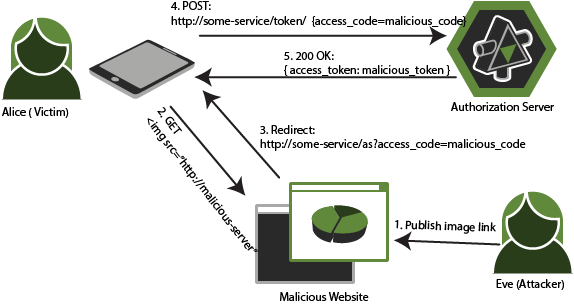
\includegraphics[scale=0.65]{chapters/images/chp4/csrf.png}
    \caption[CSRF on Oauth2]{CSRF on Oauth2.\\\hspace{\textwidth}Source:\hspace{0.2cm}\url{https://stackoverflow.com/a/42520213}}
    \label{fig:csrf}
\end{figure}

\vspace{1.5cm}

To avoid this attack, the client application must make use of the \texttt{state} param.
In order to protect the client application against CSRF, the developer must implement the ability to verify whether the authorization codes or access tokens issued to it are valid (that is, they are the result of a valid authorization request by the user from the client application). To do this, the client application must generate a session-specific, unguessable value that it can pass along with its authorization request. When an authorization code or access token is returned back to the redirect URI, the application can validate that value to ensure that it was indeed used as part of a valid authorization request initiated by the user, and not by some attacker.

If a \texttt{state} param value is passed to a service provider, the OAuth2 specification mandates that it MUST be returned back to the client application untouched. This mechanism is designed specifically to mitigate such CSRF attacks, and should be used particularly for this reason.

\subsubsection{Phishing}
Phishing is an attack in which an attacker creates a page or application that looks similar or identical to a target site with the intention that users will be unaware that it is a duplicate and so will enter secret information, like username and password, only to be captured by the impostor site.

OAuth2 client applications are vulnerable to phishing because they rely on sending a user's user-agent to and from the service provider endpoints in order to delegate authority. When developing the client application, everyone should consider the security implications of how the users will interact with the service provider to authenticate. A good rule of thumb is to follow the best practice mentioned earlier (see \ref{native}).

If native external browsers are used in an application, users will have an increased ability to verify the authenticity of the authorization endpoint that they are seeing.

\vspace{1cm}

\begin{figure}[ht]
    \centering
    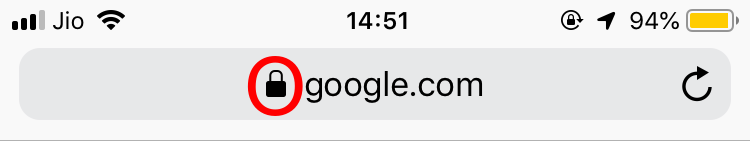
\includegraphics[scale=0.55]{chapters/images/chp4/oie_toIlpPOFRMdK.png}
    \caption{Example of site validity on Safari for iOS}
    \label{fig:ioslock}
\end{figure}

\vspace{0.5cm}

With native browsers, there are often more indicators of a site's validity (for example the lock next to the URL in iPhone's mobile Safari in Fig.~\ref{fig:ioslock}). This isn't the case with embedded browsers, which makes utilizing counterfeit pages much easier for attackers.

\subsubsection{Redirection URI manipulation}
When a client application makes an authorization request for a user, it passes along a \texttt{redirect\_uri} parameter. This parameter can be modified by an attacker, forcing the redirection to a third party URI.
Furthermore, if the application allows users to own or create a webspace of some sort that they control, like a homepage or a user profile page, they may be able to leverage it as part of their attack.

For example, considering the scenario where the application ExApp allows users to create a homepage on their domain. The user Eve may have a homepage that she controls at \texttt{www.exapp.com/users \\ /eve}. If the service provider (whith whom the app is interacting with) allows to register wildcard redirect URIs, like \texttt{www.exapp.com/\*}, or doesn't require to register a redirect URIs at all, then an attacker, such as Eve, would be able to use this homepage to her advantage.
What Eve could do is set up a fake link to log into the application, or even a counterfeit application entirely. When a user clicks on this link, they will be directed to the authorization endpoint of the service provider just as would be done from the real application. However, instead of passing the proper redirect URI, for example \texttt{www.exapp.com/callback}, this link passes her own malicious redirect URI which just happens to be her profile page, \texttt{www.goodapp.com/users/eve}. On this page, she can then intercept any authorization codes and access tokens, and proceed to impersonate users and access their protected resources.


\begin{figure}[ht]
    \centering
    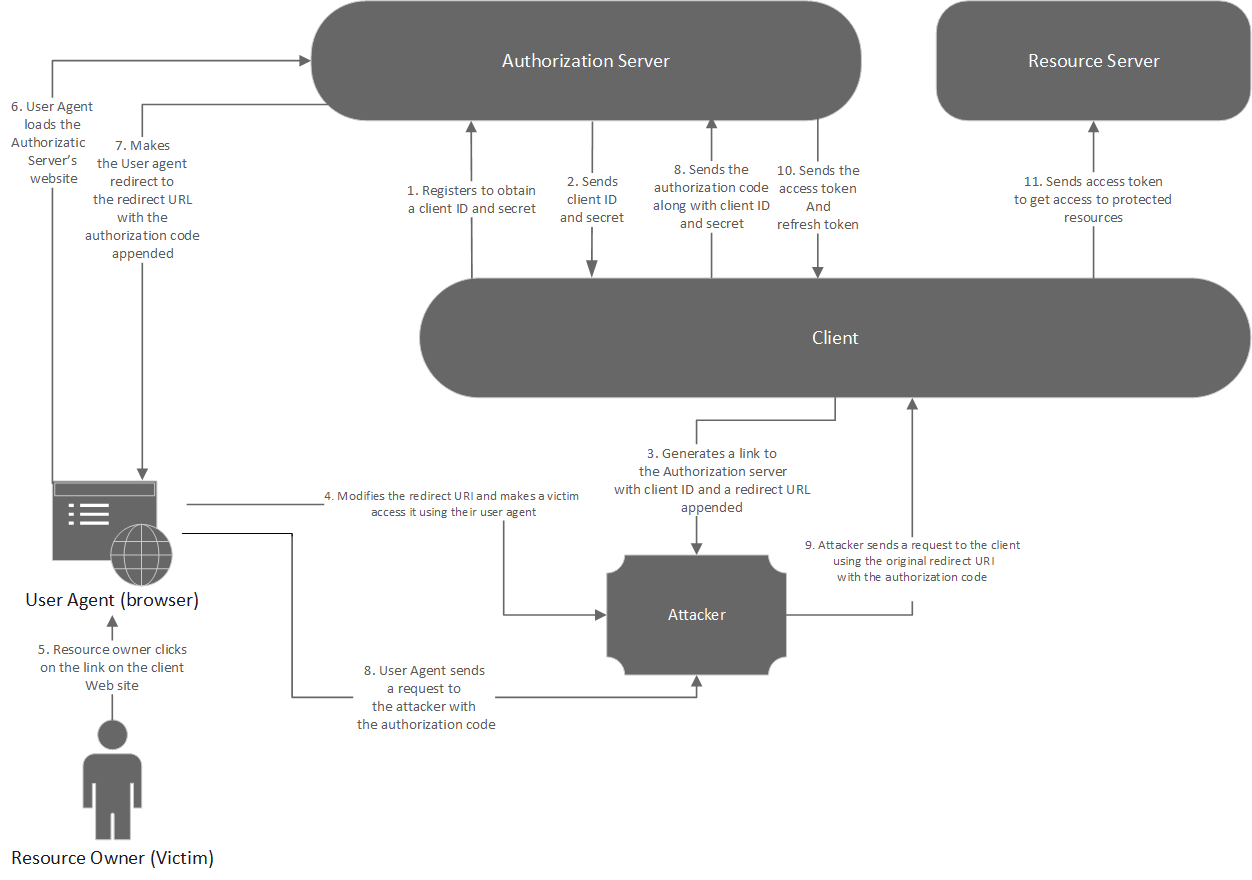
\includegraphics[scale=0.65]{chapters/images/chp4/authCodeURIAttack.png}
    \caption[Redirection URI manipulation's typical flow]{Redirection URI manipulation's typical flow.\\Source:\hspace{0.2cm}\url{https://www.thearmchaircritic.org}}
    \label{fig:reduri}
\end{figure}

It must be noticed that all Eve needs to do is convince a user to follow her malicious authorization link containing her attacker-controlled redirect URI. From the user's perspective, the user experience would be mostly the same since all that is different is the redirect URI (the attacker may choose to request additional scopes too).

To mitigate this, redirect URIs must be registered. If the service provider with whom the application is interacting with allows to register wildcard redirect URIs, they must be used sparingly. Furthermore, it should always choose to prefer to register fully-qualified redirect URIs over wildcard redirection endpoints. This is especially true if the service or application allows users to create a webspace that they control, like a homepage or profile page.

\subsubsection{Client and user impersonation}
A very basic attack that is often done is simple client or user impersonation.

In client impersonation, an attacker masquerades as the client application in order to gain access to the user's protected resources. This can be achieved quite simply if an attacker is able to get access to the client credentials (that is, the client ID and client secret). With this, they would be able to impersonate the client to the service provider and to end users.

In user impersonation, an attacker will masquerade as the end user. This can be done if an attacker is able to gain access to an issued access token. With this, they would be able to make requests to the service provider to access protected resources on behalf of the user, just as the application does.

To mitigate both of these attacks, the solution is simple: protect the client credentials, codes, and tokens from end users. If an attacker were able to see any of those, they would be granted the ability to impersonate the client application or the users, or both.


